\documentclass{school-22.101-notes}
\date{October 26, 2011}

\begin{document}
\maketitle


\topic{Phase Shifts}
We want to show that phase shift converges; that is, if we fix $k$, and an increasing $l$ should lead to a decreasing $\delta_l$. 

A phase shift $\delta_l$ is defined in the above section in Eq.~\ref{delta_l}. We can determine $\delta_l$ analytically \footnote{try using the trigonometry $\sin(a+b) = \sin(a) \cos (b) + \cos(a) \sin(b)$?}. Keep in mind that $\delta_l$ is the phase shift for each of the partial wave that can scatter. It is a result of a partial wave interacting with the potential.  
\begin{figure}[ht]
    \centering
    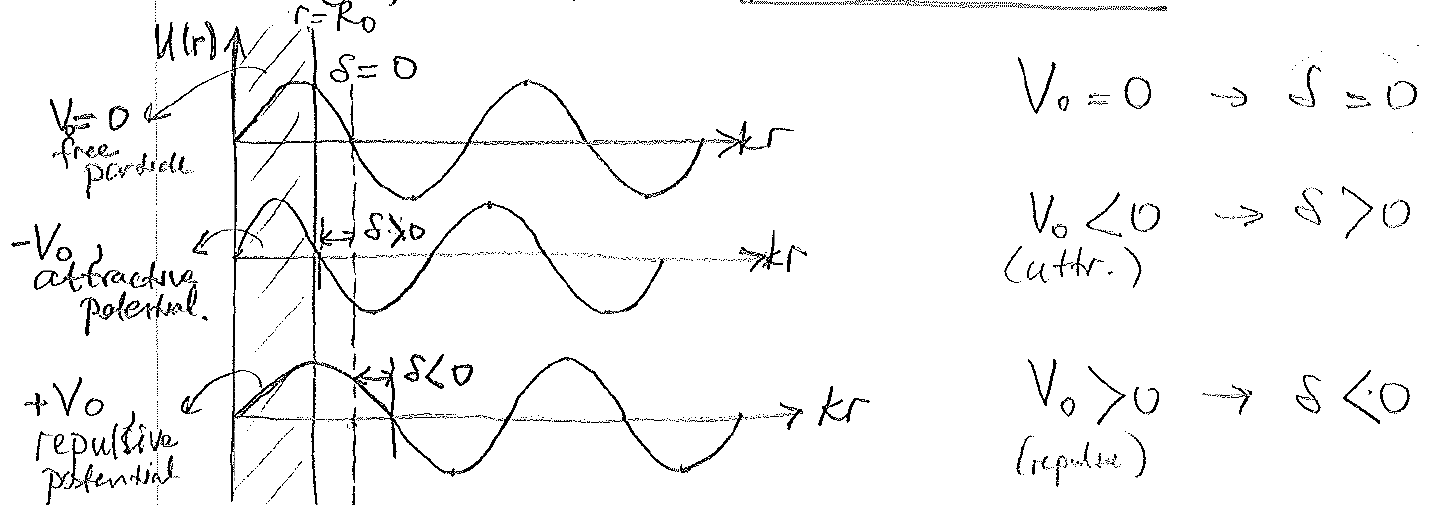
\includegraphics[width=6in]{images/scattering/scattering-potential-phase-shift.png}
    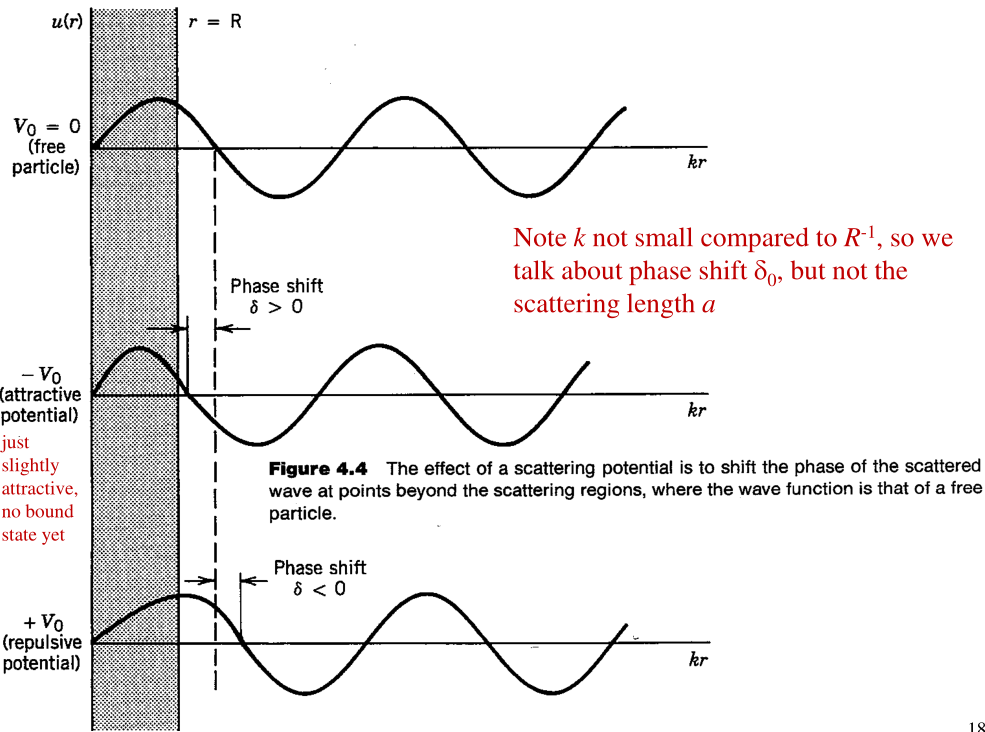
\includegraphics[width=6in]{images/scattering/scattering-potential-phase-shift-2.png}
    \caption{Phase Shift, Scattering Length }
\end{figure}




\topic{Low Energy S-Wave Approximation ($l=0$)}
\begin{figure}[ht]
    \centering
    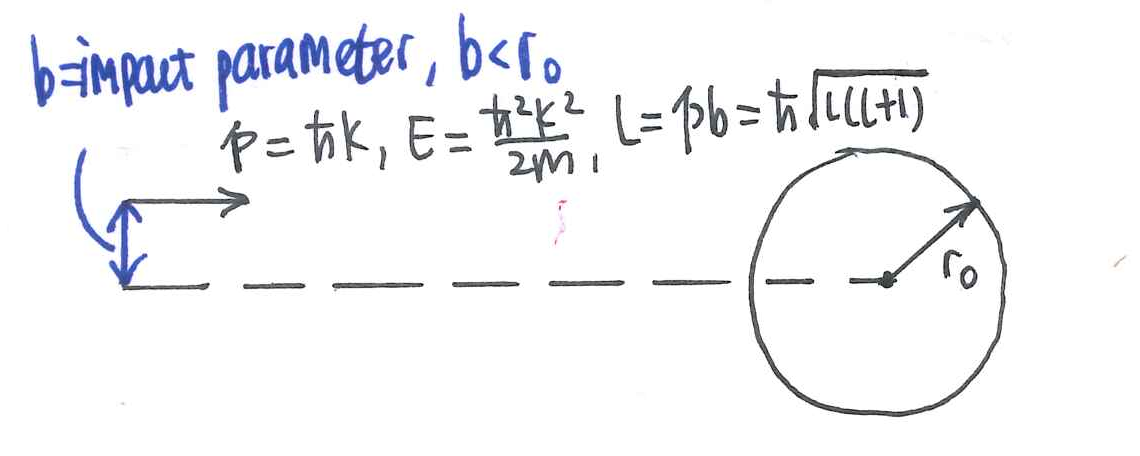
\includegraphics[width=4in]{images/scattering/np-scattering-diagram.png}
    \caption{n-p Scattering Diagram, S-Wave Approximation}
\end{figure}
\begin{enumerate}
\item A particle coming with a small incoming energy E means $k r_0 \ll 1$. This is because $E = \frac{\hbar^2 k^2}{2m} \Rightarrow k = \frac{\sqrt{2mE}}{\hbar}$, so when $E$ is small, $k$ is small. Similarly $r_0$ is reasonably small as well, hence $k r_0 \ll 1$. 

\item $ p = \hbar k$. 

\item $l=0$ because $l<kr_0 \ll 1$:
\begin{align}
L &= pb = \hbar \sqrt{l (l+1)} \approx \hbar l \Rightarrow \hbar l = pb = \hbar k b \\
\Rightarrow b &= \frac{l}{k} < r_0 \Rightarrow l < kr_0 \\
l &< k r_0 \ll 1 \Rightarrow l = 0
\end{align}

\item This is called a S-Wave Approximation. $\sigma (\theta), \sigma$ are simplified when $l=0$:
\begin{align}
\sigma (\theta) &= \frac{1}{k^2} \sin^2 \delta_0 & \sigma &= \boxed{ \frac{4 \pi}{k^2} \sin^2 \delta_0 } \label{sigma}
\end{align}

\item Observation: $\sigma$ is spherically symmetric, isotropic, because we assumed no $\theta$ dependency in S-Wave approximation. Example: when $E \approx 1 \fsp \eV \sim 10^4 \fsp \eV, \sigma = 20 \fsp b$. 

\item \textbf{Scattering Length $a$}: In the limit of low E, we define scattering length as\footnote{$a$ may be positive or negative. Here we use Krane's notation.}:
\begin{align}
\left. \begin{array}{c}
- \lim_{k\to 0} f(\theta) = a  \\
f(\theta) = \frac{1}{k} \Sum (2l+1) e^{i \delta_0} \sin \delta_0  P_l (\cos \theta) = \frac{1}{k} e^{i\theta_0} \sin \theta_0  \approx \frac{\delta_0}{k} 
\end{array} 
\right\} \Rightarrow \delta_0 = -ak
\end{align}
\begin{align}
\sigma &= 4 \pi \frac{1}{k^2} \sin^2 \delta_0 \approx 4 \pi \frac{\delta_0^2}{k^2} =  4 \pi \frac{(-ak)^2}{k^2} = 4 \pi a^2 \\
u(r) &= \frac{A_0}{k} \sin(kr + \delta_0) = \frac{a_0}{k} \sin (k(r-a)) \xrightarrow{\mathrm{small \fsp k}} \frac{a_0}{k} (k(r-a))
\end{align} 
The above expression suggests that $a$ behaves like an intercept as in Fig.~\ref{scattering-s-wave}. 

\begin{figure}
  \centering
    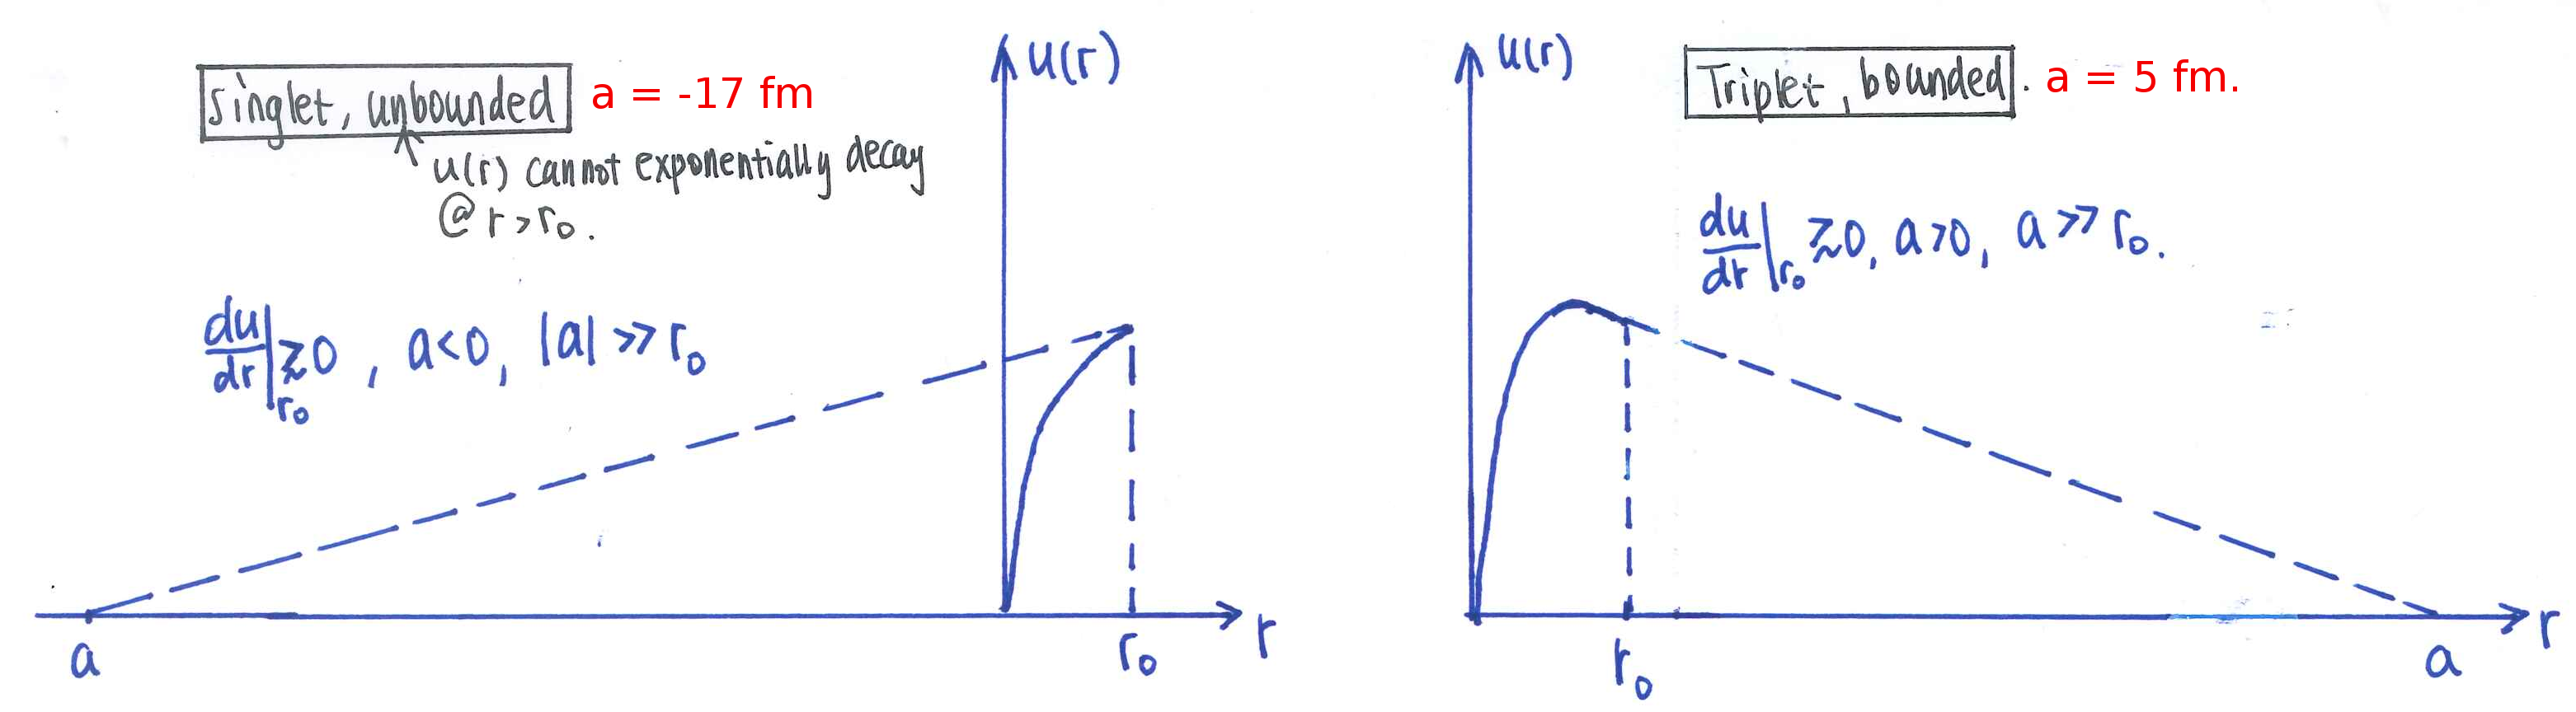
\includegraphics[width=7in]{images/scattering/s-wave-singlet-triplet.png}
    \\
    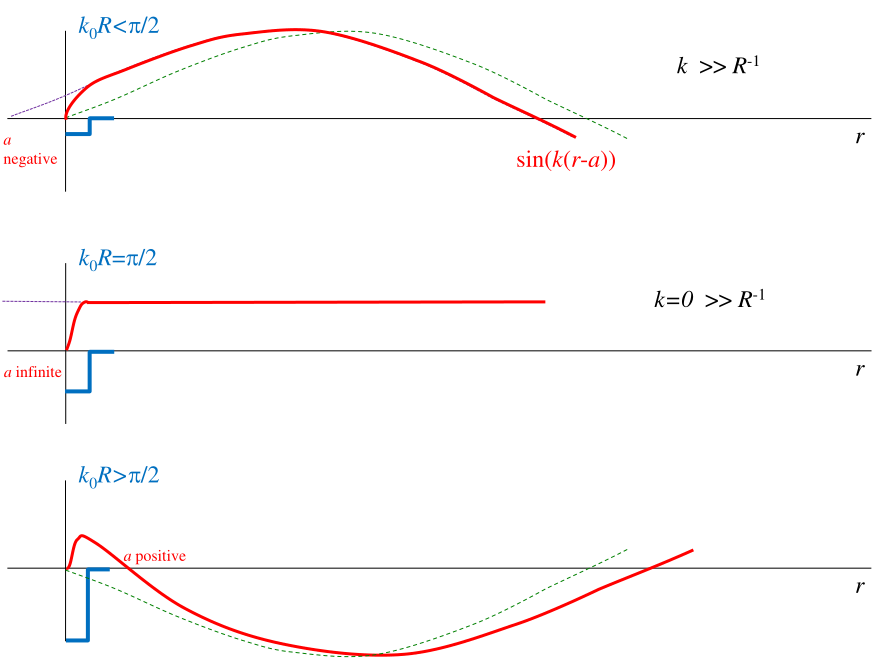
\includegraphics[width=5in]{images/scattering/s-wave-singlet-triplet-2.png}
    \caption{Singlet vs. Triplet Configuration for Low Energy ($E<10 \fsp \mathrm{keV}$)\label{scattering-s-wave}}
\end{figure}

Implications of Figure~\ref{scattering-s-wave}:
\begin{enumerate}
\item Sign of $a$:  positive $a$ refers to triplet/bound state, negative $a$ refers to singlet/unbounded state. 
\item $a \gg r_0$. 
\item $a$ is `scattering amplitude' because 
\eqn{ \psi_{\mathrm{sc}} = f_0 \frac{e^{ikr}}{r} = \frac{\delta_0}{k} \frac{e^{ikr}}{r} = -a \frac{e^{ikr}}{r}  }
\end{enumerate}
\end{enumerate}

\uline{Alternative approach to low energy s-wave} presented by Prof. Li on 10/24/12: as $k\to 0$, only $l=0$ term is important. The SEQ is, 
\eqn{ (\laplacian + k^2) \psi(x) = \frac{2 \mu V(x) \psi(x)}{\hbar^2} } 
Then we arrive at the Lippmann-Schwinger equation, 
\eqn{ \psi(x) = e^{ikx} - \int \dx'^3 \frac{e^{ik|x-x'|}}{4\pi |x-x'|} \frac{2 \mu V(|x'|) \psi(x') }{\hbar^2} }
Notice we arrive at an equation of $\psi(x)$ that depends on $\psi(x)$. We iterate, that is, we plug $\psi(x') = e^{ikx'}$ to solve for $\psi(x)$ and plug back in again. If we only iterate once and ignore $O(V^2)$, then we arrive at the \textbf{First Boron Approximation}, 
\eqn{ \psi(x) = e^{ikx} - \int \dx'^3 \frac{e^{ik|x-x'|}}{4\pi |x-x'|} \frac{2 \mu V(|x'|) e^{ikx'} }{\hbar^2} }
In the limit of low energy scattering ($k \to 0$), the wave is of central/spherical, that is, $f(\theta)$ is a constant. More specifically, we can see that in low energy s-wave approximation, 
\eqn{ \lim_{k\to 0} f(\theta) = \lim_{k\to 0} \frac{1}{k} e^{i\delta_0} \sin \delta_o = \frac{\delta_0}{k} }
We define a scattering length $a$ that satisfies 
\eqn{ a = \lim_{k\to 0} \frac{-\delta_0}{k} }
Thus $f(\theta) = -a$. Then the wavefunction is, 
\eqn{ \psi (x) = e^{ikx} - a \frac{e^{ikr}}{r} }
and the total scattering cross section is,
\eqn{ \sigma = \lim_{k\to 0} 4 \pi \frac{\delta_0^2}{k^2} = 4 \pi a^2}


Next we consider many scatters. We assume that there is no overlap between different scatters, and the scatterings are well separated, so we can use superposition. The wavefunction comes out to be,
\eqn{ \psi(x) = e^{ikx} - \left[ \Sum_m a_m e^{i (k-k_{\mathrm{out}}) \cdot x_m} \right] \frac{ e^{ikr}}{r} }
Comments: 
\begin{itemize}
\item Many scatters are not isotropic anymore because of the interference. 
\item The sign of $a$ does not matter for $\sigma$ in the case of single scatter. But with multiple scatters, the signs of each $a$ would matter. 
\item We define a $\displaystyle q = k_{\mathrm{out}} - k = k(\hat{x} - \hat{e}_z), S(q) = \Sum_m a_m e^{-i q \cdot x_m}$, so 
  \eqn{ \psi_{\mathrm{scatter}} (x) = - S(q) \frac{e^{ik|x|}}{|x|} }
  This is the basis of particle scattering. Setting up detectors at different location would tell us information about the structure of the nuclides. The readings on the detector is the intensity $I(q) \propto |S(q)|^2$. 
\end{itemize}
We consider the well problem again and solve the SEQ. After derivation,  
\eqn{ R - a &= \tan (k_0 R) / k_0 & a &= R - \frac{\tan(k_0 R)}{k_0} }
We can plot $a$ as a function of $k_o R$ as in Fig.\ref{scattering-s-wave} and observe:
\begin{itemize}
\item $V_0 = 0, k_0 = 0, \Rightarrow a= 0 ,\sigma = 0$. 
\item As $V_0 \up, k_0 \up, a$ becomes negative during $\displaystyle k_0 R \in \left[0, \frac{\pi}{2} \right]$. 
\item $k_0 R = \frac{\pi}{2}, a = -\infty, \sigma = \infty$, we hit resonances as in Fig.~\ref{low-energy}. A subtle point here is that the curve ($a$ vs. $k_0 R$ which is effectively cross section as a function of well depth) looks very similar to the resonance scattering cross section plot with respect to energy. While the two plots are not quite the same thing, they do have the same underlying principle in the sense that $E$ and $V$ show up in the SEQ as a single term $E-V$.  
\item $k_0 R \in [\frac{\pi}{2}, \pi]$, $a$ is positive. 
\item $k_0 R$ approaches $\pi$, $a = 0$, the particle is effectively invisible. 
\end{itemize}
\begin{figure}[ht]
\centering
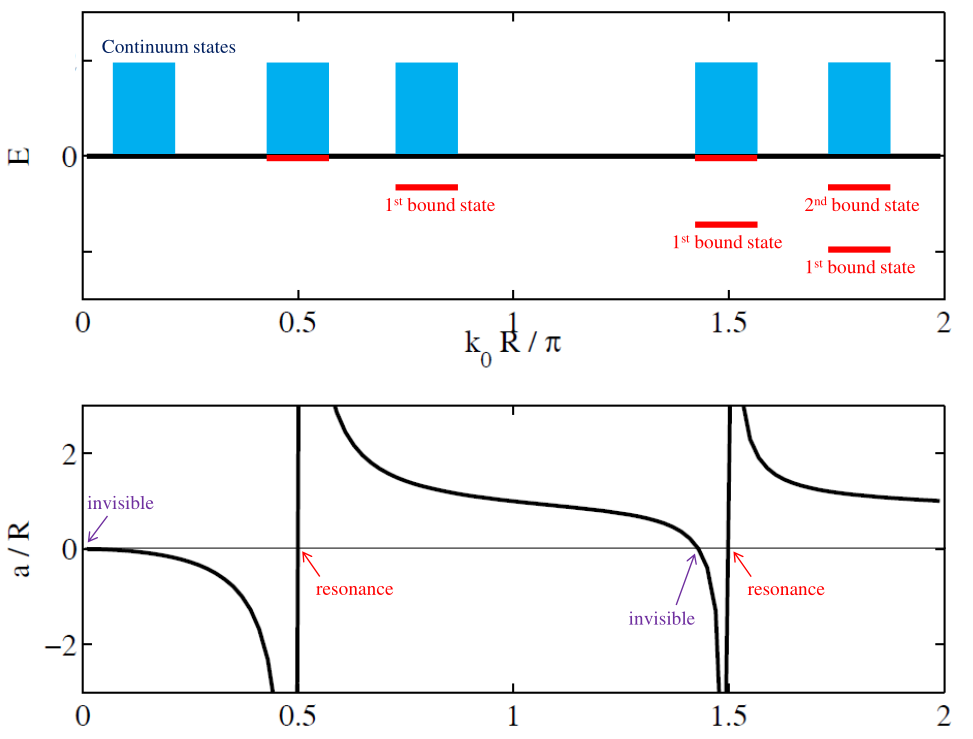
\includegraphics[width=5in]{images/scattering/low-energy.png}
\caption{Low Energy Scattering} \label{low-energy}
\end{figure}




\topic{Application of S-wave: n-p Scattering}
We apply S-wave approximation to n-p scattering in a Finite Square Well with $-V_0$ potential:
\begin{align}
\begin{cases}
u(r) = A \sin(k_1 r) & r \le r_0, k_1 = \frac{\sqrt{2 \mu (E+V_0)}}{\hbar} \\
u(r) = C \sin(k_2 r + \delta_0) & r > r_0, k_2 = \frac{\sqrt{2 \mu E}}{\hbar} 
\end{cases}
\\
\boxed{k_1 \cot (k_1 r_0) = k_2 \cot (k_2 r_0 + \delta_0) } \label{relation}
\begin{cases}
A \sin (k_1 r_0) = C \sin (k_2 r_0 + \delta_0) & u_1(r_0) = u_2(r_0) \\
A k_1 \cos (k_1 r_0) = C k_2 \cos (k_2 r_0 + \delta_0) & u^{\prime}_1 (r_0) = u_2^{\prime} (r_0) 
\end{cases}
\end{align}
Combine the transcendental relation Eq.~\ref{relation}, and the cross section relation Eq.~\ref{sigma} ($B$ means bound state, $E$ is the energy of the neutron, $E_B$ is the binding energy. ):
\begin{align}
k_2 r_0 + \delta_0 &= k_2 r_0 - ak_2 \approx -ak_2 \approx \delta_0 \\
\mathrm{RHS} &= k_2 \cot (k_2 r_0 + \delta_0) \approx k_2 \cot (\delta_0) \\
k_1 \cot (k_1 r_0) &\approx k_1^B \cot (k_1^B r_0) = - k_2^B  = k_2 \cot (\delta_0) \\
\cot (\delta_0) &= -\frac{k_2^B}{k_2} \\
\sin^2 (\delta_0) &= \frac{1}{1 + \cot^2 (\delta_0)} = \frac{1}{1 + \left( \frac{k_2^B}{k_2} \right)^2 } = \frac{k_2^2}{k_2^{B2} + k_2^2} \\
\sigma &= \frac{4\pi}{k_2^2} \sin^2 (\delta_0) = \frac{4\pi}{k_2^2 + \left(k_2^B \right)^2 } = \frac{4\pi \hbar^2}{2 \mu (E + E_B) } \xrightarrow{E \ll E_B} \frac{4 \pi \hbar^2}{2 \mu} \frac{1}{E_B} \\
&\xrightarrow{E_B = 2.22 \mathrm{ MeV}} 2.3 \mbox{ b} 
\end{align}
Notice $\sigma (\theta) = 2.3$ b is significantly smaller than the measured 20 b. The missing piece is the spin-spin coupling component.

\textbf{Spin-spin Coupling}: Recall $S=0$ is singlet with P=1/4, $S=1$ is triplet with P = 3/4. 
\begin{align}
\sigma( \theta) &= \frac{3}{4} \sigma_T (\theta) + \frac{1}{4} \sigma_S (\theta) = \frac{3}{4} \frac{1}{k_2^2} \sin^2 (\theta_{ot} ) + \frac{1}{4} \frac{1}{k_2^2} \sin^2 (\theta_{os} ) \\
\sigma &= 4 \pi \sigma (\theta) = \frac{4 \pi \hbar^2}{2 \mu} \left[ \frac{3}{4} \frac{1}{E_B} + \frac{1}{4} \frac{1}{E^*} \right] 
\end{align}\footnote{we can write $\sigma = 4 \pi \sigma(\theta)$ because l=0 is symmetric potential, so we don't need to integrate here} 
Plug in $E_B = 2.22 \fsp \MeV, E^* = 0.077 \fsp \MeV$, $\sigma = 19$ b, which is a good approximation for 20b. 



\topic{Spin Dependence of Nuclear Force} \label{spin-scattering}
This lecture is presented by Prof. Li on 10/31/12). Refer to Section~\ref{2H-spin} on some previous coverage on spin dependence in bound state. We consider shotting a neutron at a neutron, shotting a proton at a neutron, shotting a proton at a proton. We use the notation `singlet' when the incoming particle's and the stationary particle's spins are misaligned, $S=0$; `triplet' when the incoming particle's and the stationary particle's spins are aligned, $S=1$. 
\begin{enumerate}
\item $\displaystyle a^{\mathrm{singlet}}_{nn} = -16.6 \fm$. 
\item $\displaystyle a^{\mathrm{singlet}}_{pp} = -7.82 \fm$. If we remove the Coulomb effect, $\displaystyle \tilde{a}^{\mathrm{singlet}}_{pp} = -17.1 \fm \sim a^{\mathrm{singlet}}_{nn}$. This is called `charge' symmetry. 
\item $\displaystyle a^{\mathrm{singlet}}_{np} = -23.72 \fm$ (which is called `nearly charge' independence because it is close to $a^{\mathrm{singlet}}_{nn}$). $\displaystyle \sigma_{S=0} = 67.8$ barn. 
\item $\displaystyle a^{\mathrm{triplet}}_{np} = 5.423 \fm$. There is only 1 weakly bound state. $\displaystyle \sigma_{S=1} = 4.6$ barn. 
\end{enumerate}

The fact that $\sigma_{S=0} \neq \sigma_{S=1}$ implies that nucleon-nucleon force is spin-dependent. We consider the Hamiltonian operator and consider the following three spin dependences: 
\begin{enumerate}
\item Spin-spin dependency(see Eq. 4.48 in Krane). 
\begin{align}
 \frac{\expect{s_1 \cdot s_2}}{\hbar^2} &= \expect{\frac{S^2 - S_1^2 - S_2^2}{2 \hbar^2}}  =  \expect{\frac{S(S+1) - \frac{1}{2} \frac{3}{2} 2 \hbar^2}{2 \hbar^2} } = \left\{  \begin{array}{cc} - \frac{3}{4} & S = 0 \\ \frac{1}{4}  & S= 1 \end{array} \right. \\
V_{ss} (r) &= V_1 (r) \left( \frac{1}{4} - \frac{S_1 \cdot S_2}{\hbar^2} \right) + V_3 (r) \left( \frac{3}{4} + \frac{S_1 \cdot S_2}{\hbar^2} \right)
\end{align}
Spin-spin dependence gives us $V_1(r)$ for singlet and $V_3(r)$ for triplet as in Fig.~\ref{total}, and both are attractive.


\item Spin-orbit dependency (velocity dependency). Before we consider the spin-orbit effect, the unpolarized beam behaves as in Fig.~\ref{un-spin-orbit}. Adding the spin-orbit term: $\displaystyle V_{so}(r) = V (r) (L \cdot S)$. Spin polarizer that breaks the left and right symmetry: there is a concentration effect to the neutrons coming in with up spin to move upwards as shown in Fig.~\ref{spin-orbit}(notice the up and down arrows correspond to out of the paper and into the paper as we are considering a top view). $V_{so}(r)$ is a negative term as illustrated in Fig.~\ref{total}. 

  \begin{figure}[ht]
    \centering
    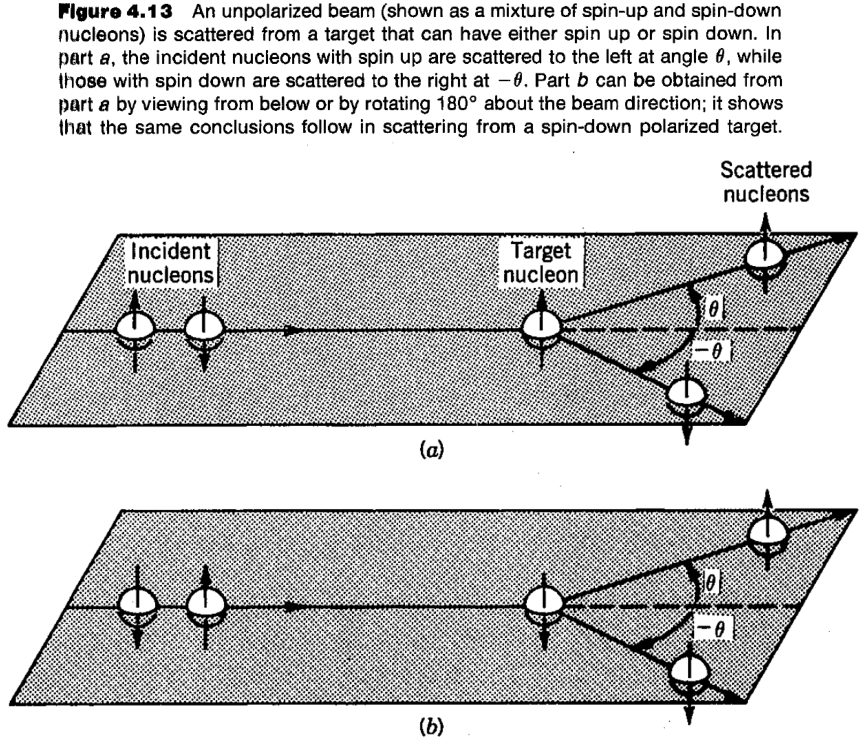
\includegraphics[width=4in]{images/scattering/un-spin-orbit.png}
    \caption{Scattering Experiment: Unpolarized Beam} \label{un-spin-orbit}
  \end{figure}

  \begin{figure}[ht]
    \centering
    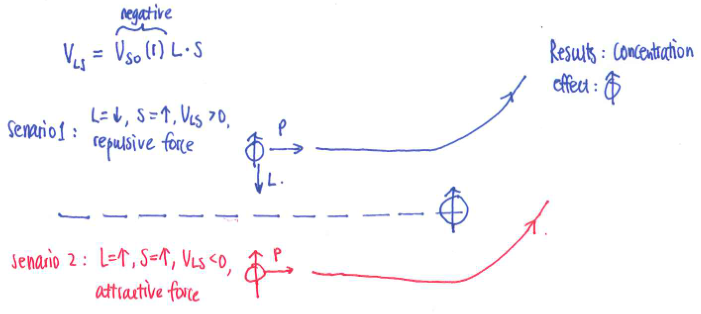
\includegraphics[width=4in]{images/scattering/spin-orbit.png}
    \caption{Scattering Experiment: Polarized Beam Due to Orbit-Spin Dependence} \label{spin-orbit}
  \end{figure}

\item Tensorial-spin dependency for bounded deuteron. From electric quadrupole measurements, we observe that deuteron with $I = 1, S=1$ is 96\% s-wave bound state ($l=0$), 4\% d wave ($l=2$). We know that $l=1$ is forbidden from $\pi = (-1)^l = 1^+$, so $l$ can only be even. Then the tensorial force: 
\eqn{ V_T(r) = V \left[ 3 \frac{(s_1 \cdot x) (s_2 \cdot x)}{|x|^2} - s_1 \cdot s_2 \right] }
where the $3 \frac{(s_1 \cdot x) (s_2 \cdot x)}{|x|^2}$ is non-centripetal (because a centripetal force should only be depend on $x^2$) and this term gives the d-wave characteristics.  The tensor force term breaks the conservation of orbital angular momentum, but does not break parity symmetry. The existence of this tensor force means that the real nucleon-nucleon potential is actually not central. But since $V_T(r)$ is not so large, the central potential model is still a good approximation. 
\end{enumerate}

\begin{figure}[ht]
  \centering
  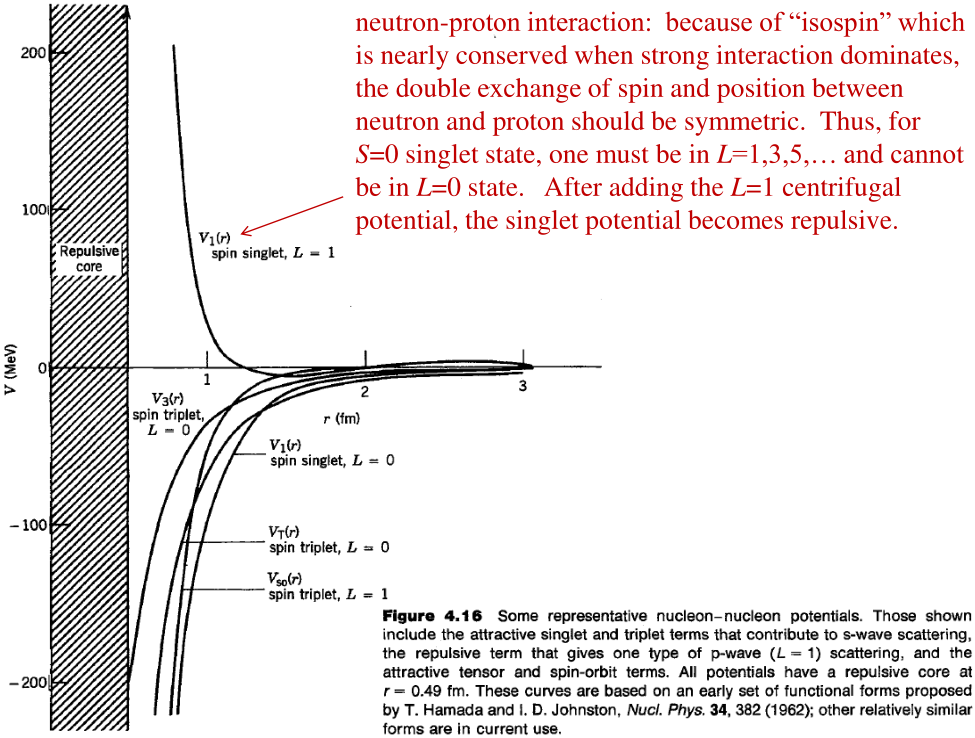
\includegraphics[width=5in]{images/scattering/total-spin-dependency.png}
  \caption{Nucleon-nucleon Potential Demonstrating How the Spin Dependency Changes the Potentials} \label{total}
\end{figure}

Fig.~\ref{total} put the three pieces together. Comments:
\begin{itemize}
\item There is an approximate isospin symmetry between a neutron and a proton, that is, if we double swap the position and the spin of a neutron with a proton, we should preserve the symmetry. 

\item Why a deuteron bound state cannot be singlet? Given $S=0, \pi = -1$, then $L$ has to be odd. Thus we have to adjust the singlet state by adding in a centrifugal term: $V_1(r) \to V_1(r) \frac{l(l+1)}{r^2}$, and it's this centrifugal term that makes the singlet state potential positive (repulsive) as in Fig.~\ref{total}, not the original singlet (`naked singlet' as Prof. Li calls it) that is repulsive. 

\item A neutron and a proton cannot be closer than 0.5 fm at any given time; thus it is called a repulsive core in Fig.~\ref{total}. 
\end{itemize}



%%%%%%%%
\topic{Summary} 
Nuclear force properties: 
\begin{enumerate}
\item Strongly attractive at short distances. It provides the overall shell-model potential.
\item At range on the order of the nuclear radius, the force distorts the nucleus. 
\item At range much smaller than the nuclear radius, the force makes the nucleus spherical and pairs up nucleons.
\item Strongly spin dependence:
    \begin{enumerate}
    \item Spin-spin interaction: $V(r) = V_0(r) + V_1 (r) \frac{\Shat_1 \cdot \Shat_2}{\hbar^2} $, $\sigma_S \neq \sigma_T$
    \item Spin-orbit interaction.
    \item Tensorial-spin interaction. 
    \end{enumerate}    
\item Nearly charge-independent (Coulomb interaction excluded).
\item The force saturates.
\end{enumerate}



\end{document}
